\section{Heat transport}

File: \texttt{07\_heat.yaml}

\subsection{Description}

The task is inspired by the hot-dry-rock method of geothermal heat
exchanger. The exchanger should be in progress for 30 years and give the
power of 25 MW.

The user will learn how to:

\begin{itemize}
\tightlist
\item
  Set up heat transfer model;
\item
  Use transition parameters at interfaces;
\item
  Specify linear algebra solver.
\end{itemize}

\subsection{Input}

\subsubsection{Geometry}

We consider a two-dimensional model 5000 \(\times\) 5000 m with two
vertical wells at the distance of 3000 m. The wells are 4300 m deep with
the diameter approx. 11 cm (Figure \ref{fig:BCD}). In order to better
capture the 3D nature of the problem, we set \texttt{cross\_section}
(width) of the rock region to 100 m (the value was gained from
calibration), and the cross section of the wells to 0.04 m\({}^2\).

\begin{longtable}[c]{@{}lr@{}}
\caption{Geometrical parameters.
\label{tbl:water_balance}}\tabularnewline
\toprule
Parameter & Value\tabularnewline
\midrule
\endfirsthead
\toprule
Parameter & Value\tabularnewline
\midrule
\endhead
Model width & 5000 m\tabularnewline
Model depth & 5000 m\tabularnewline
Depth of heat exchanger & 4100 -- 4300 m\tabularnewline
Distance of wells & 3000 m\tabularnewline
Depth of wells & 4200 m\tabularnewline
Model cross section & 100 m\tabularnewline
Well cross section & 0.04 m\({}^2\)\tabularnewline
\bottomrule
\end{longtable}

\begin{figure}[htbp]
\centering
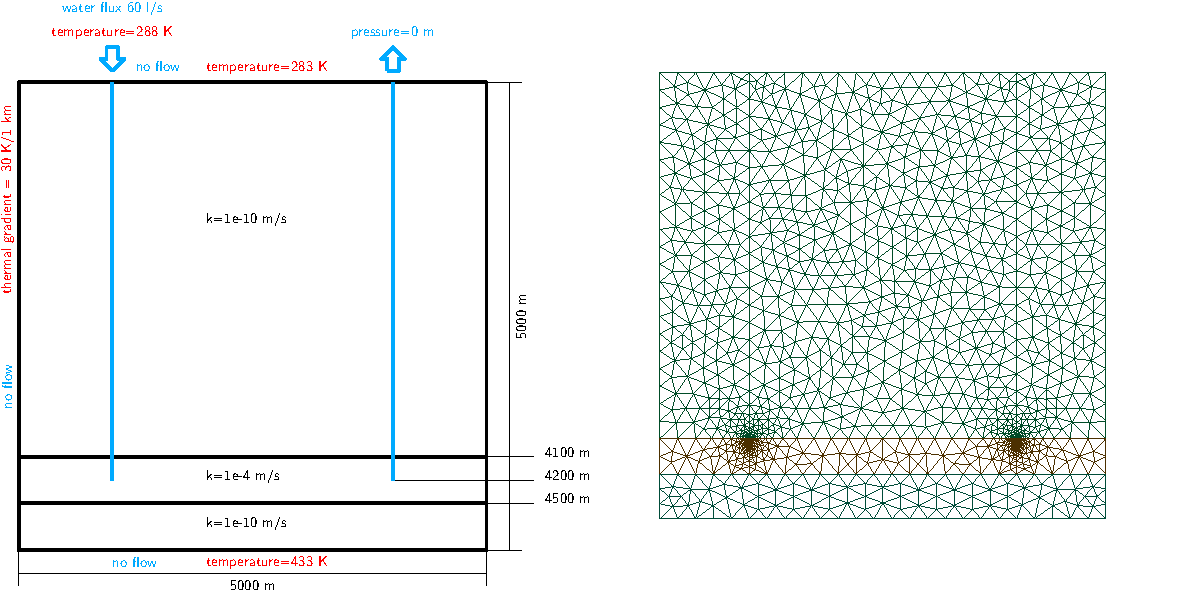
\includegraphics[width=1.00000\textwidth]{tutor_figures/07_bcmesh.pdf}
\caption{Geometry, boundary conditions and computational
mesh.\label{fig:BCD}}
\end{figure}

\subsubsection{Hydraulic model}

The hydraulic conductivity was set to 1 \(\times\) \(10^{-10}\) m/s for
the rock and to 1 \(\times\) \(10^{-4}\) m/s for the exchanger zone.

\begin{verbatim}
  - region: rock
    cross_section: 100
    conductivity: 1.0e-10
  - region: exchanger
    conductivity: 1e-4
\end{verbatim}

The flow in the wells is modelled using the Darcy equation with a high
hydraulic conductivity (10 m/s). The transition coefficient
\texttt{sigma} {[}--{]}, determines the rate of exchange between 2D rock
and 1D wells. Its default value 1 is kept at the lower well ends,
elsewhere the wells are isolated and hence we set \texttt{sigma} to
zero.

\begin{verbatim}
  - region: wells
    conductivity: 10.0
    cross_section: 0.04
    sigma: 0
  - region: wells_deep
    sigma: 1
\end{verbatim}

On the injection well (``.well1\_surface''), we prescribe the flux 60
l/s, i.e.~the flux velocity is 1.5 m/s. On the production well
(``.well2\_surface'') we prescribe zero pressure.

\begin{verbatim}
  - region: .well1_surface
    bc_type: total_flux
    bc_flux: 1.5
  - region: .well2_surface
    bc_type: dirichlet
    bc_pressure: 0
\end{verbatim}

We assume that the system does not have contact with its surrounding
because of high depth and intact granite massive. Hence no flow boundary
conditions are given on the sides, on the bottom and on the surface.

For the solution of the flow problem we choose the LU decomposition as
the linear algebra solver:

\begin{verbatim}
  nonlinear_solver:
    linear_solver: !Petsc
      options: -ksp_type preonly -pc_type lu
\end{verbatim}

\subsubsection{Heat transport model}

The heat transport model (\texttt{Heat\_AdvectionDiffusion\_DG}) assumes
that the fluid and solid phase are at thermal equilibrium. For the whole
model (\texttt{-\ region:\ ALL}) we prescribe the parameters for water
and granite (density, thermal conductivity and capacity):

\begin{verbatim}
  heat_equation: !Heat_AdvectionDiffusion_DG
    balance:
      cumulative: true
    input_fields:
      - region: ALL
        fluid_density: 1000.0
        fluid_heat_capacity: 4000
        fluid_heat_conductivity: 0.5
        solid_density: 2700.0
        solid_heat_capacity: 790
        solid_heat_conductivity: 2.5
\end{verbatim}

The temperature on the surface is set to 283 K (\(=10^\circ\)C):

\begin{verbatim}
  - region: .surface
    bc_type: dirichlet
    bc_temperature: !FieldFormula
      value: 10+273.15
\end{verbatim}

The injected water has temperature \(15^\circ\)C:

\begin{verbatim}
  - region: .well1_surface
    bc_type: dirichlet
    bc_temperature: !FieldFormula
      value: 15+273.15
\end{verbatim}

The temperature on the bottom and sides as well as the initial
temperature in the rock and the wells is then prescribed in agreement
with typical geological gradient, approx. \(1^\circ\)C / 33 m:

\begin{verbatim}
    init_temperature: !FieldFormula
      value: 10-z/5000*150+273.15
\end{verbatim}

The porosity was set to 1 \(\times\) \(10^{-5}\) for rock and 1
\(\times\) \(10^{-4}\) for exchanger. The transition coefficient of
wells (``fracture\_sigma'') was set to 0 in rock surrounding and to 1 in
deep surrounding:

\begin{verbatim}
  - region: wells
    init_temperature: !FieldFormula
      value: 15-z/5000*150+273.15
    porosity: 1.0e-05
    fracture_sigma: 0
  - region: wells_deep
    fracture_sigma: 1
\end{verbatim}

\subsection{Results}

The evolution of power of the heat exchanger (difference of absolute
energy flux on the surface of the two wells) is depicted in Figure
\ref{fig:tempr}. The result of water flow is depicted in Figure
\ref{fig:flux} and the temperature field of the whole massif after 30
years is depicted in Figure \ref{fig:tempr_grad}.

\begin{figure}[htbp]
\centering
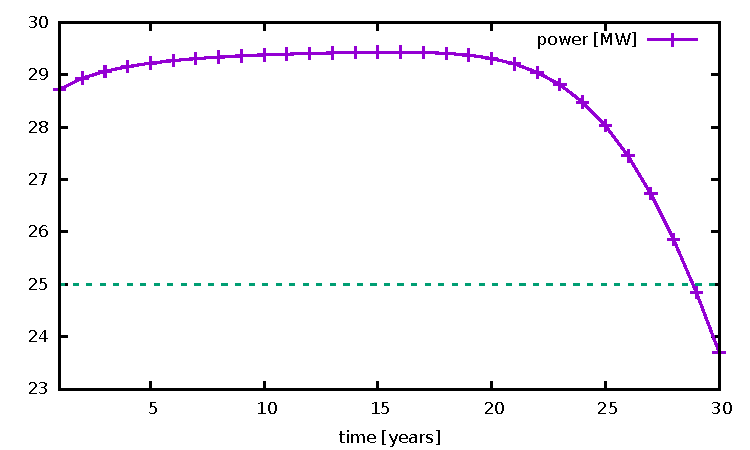
\includegraphics{tutor_figures/07_power.pdf}
\caption{The power of heat exchanger system in 30
years.\label{fig:tempr}}
\end{figure}

\begin{figure}[htbp]
\centering
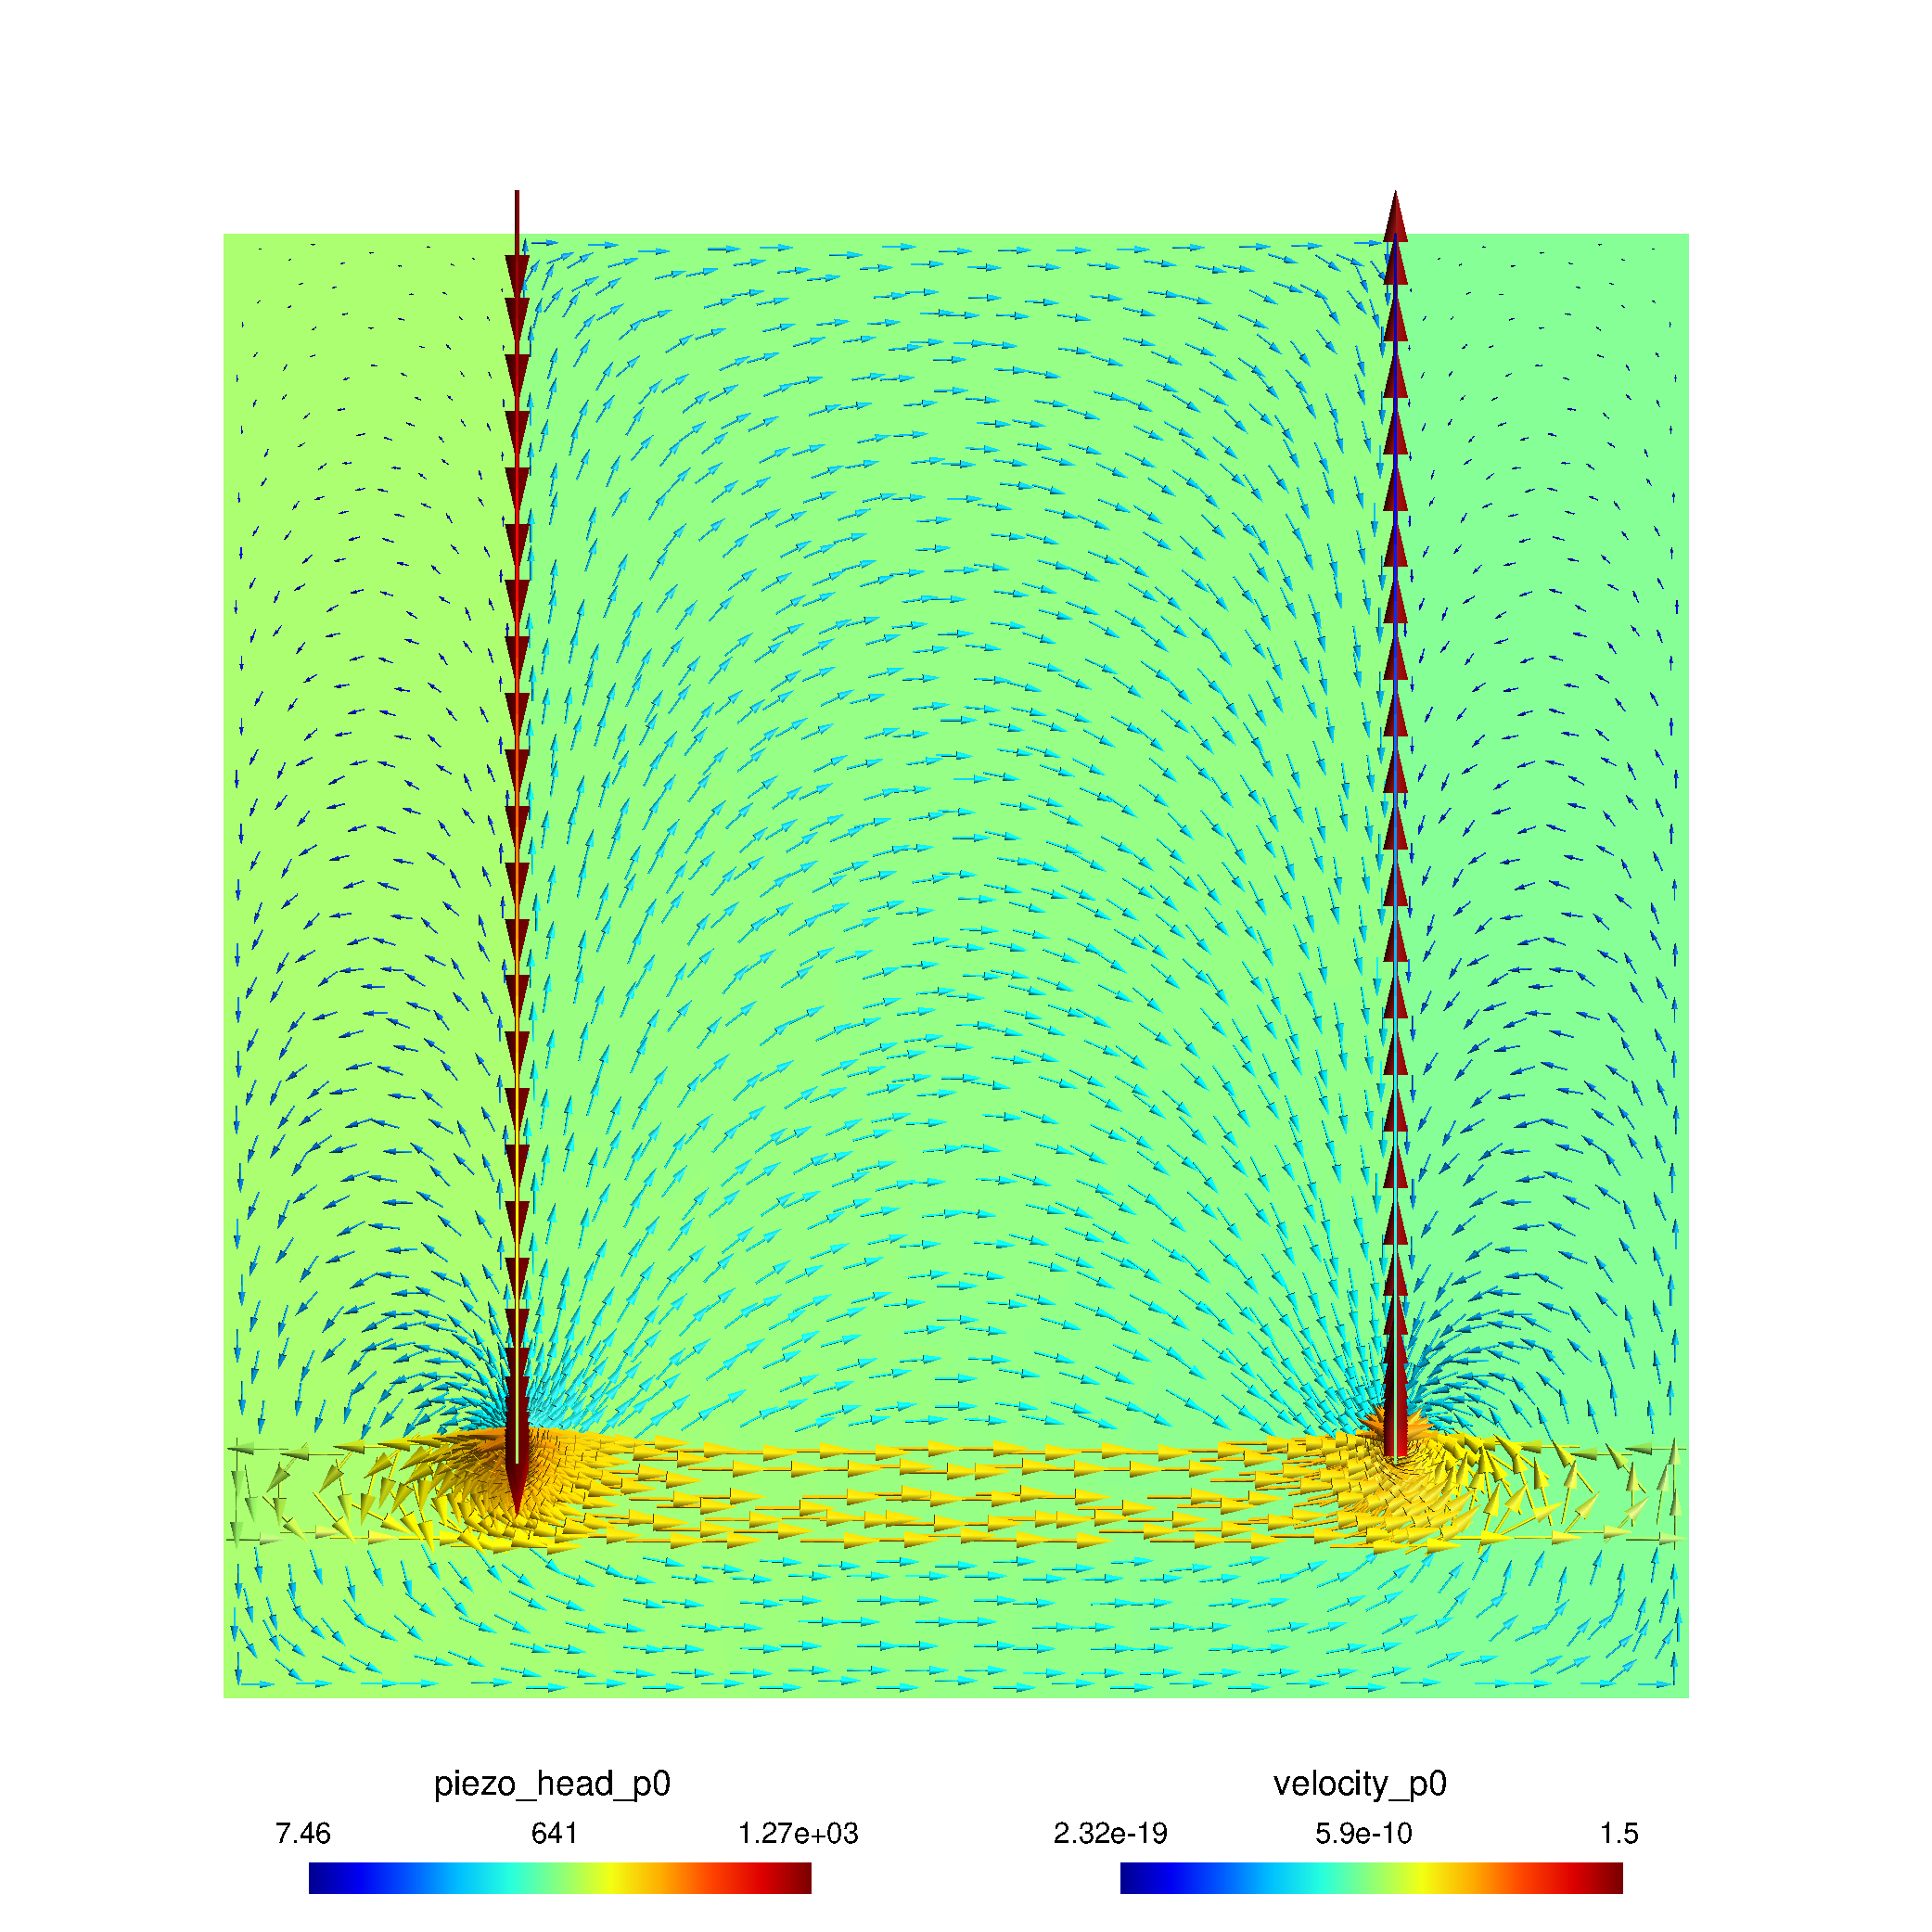
\includegraphics[width=0.80000\textwidth]{tutor_figures/07_flow.pdf}
\caption{The flux field with piezometric head.\label{fig:flux}}
\end{figure}

\begin{figure}[htbp]
\centering
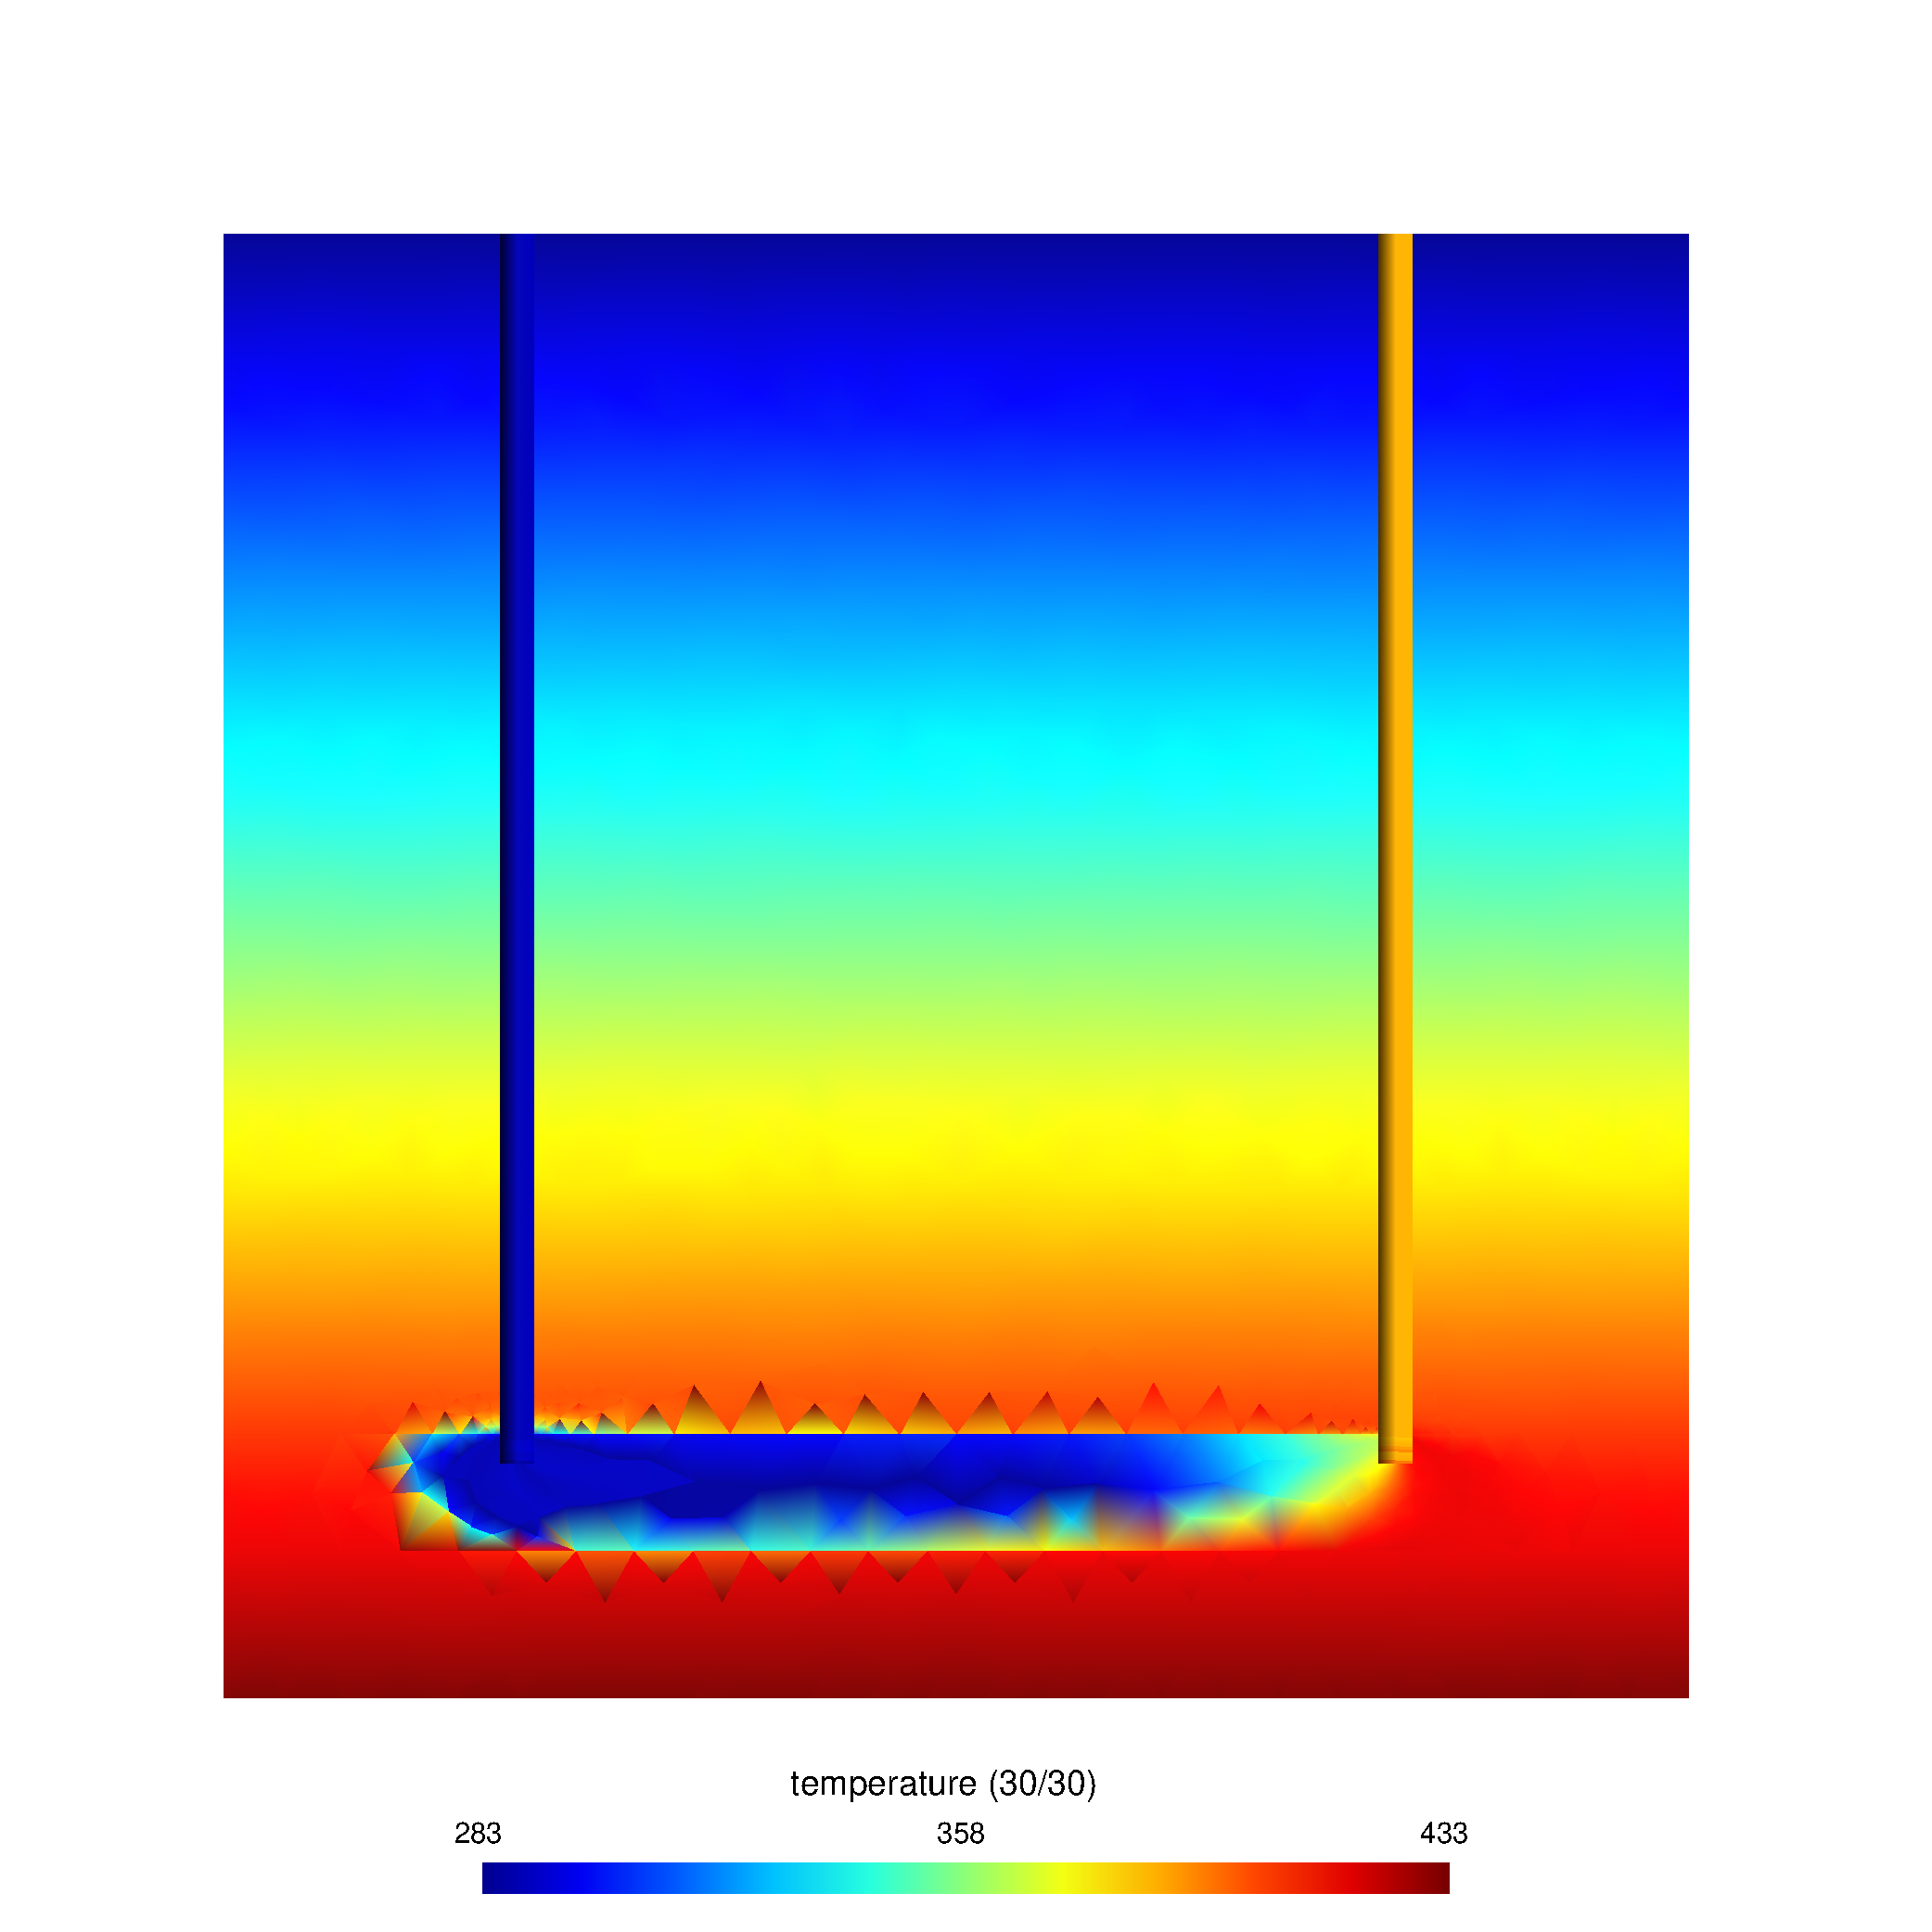
\includegraphics[width=0.80000\textwidth]{tutor_figures/07_transport.pdf}
\caption{The temperature of exchanger after 30
years.\label{fig:tempr_grad}}
\end{figure}
